\chapter{Collaboration in Immersive Virtual Environment}
\label{chapter:context}
\minitoc

\section{Introduction}
This chapter presents a general state of the art of different topics related to using immersive virtual environment for collaborative task. Being the joint interest of Virtual Reality (VR) and Computer Supported Collaborative Work (CSCW), research on Shared Virtual Environment (SVE) or Collaborative Virtual Environment becomes more and more popular.

With rapid increasing computation capacity and the development of computer network, multi-agent collaboration via computer-generated virtual space with new types of communication and interaction becomes available.

\section{Virtual Reality}
\subsection{Definition}
The term ``Virtual reality" was used to describe a certain type of sophisticated computer equipment which serves as a medium to connect users to a digitally created space before becoming a research domain, so early definitions of virtual reality are often device-oriented \citep{Steuer1995Defining}. 

\citep{Lanier1992VR}; \citep{Rheingold1991VR}; \citep{Sutherland1968Hmd}.



\citet{Fuchs2011Book} give a technical definition of virtual reality: ``Virtual reality is a scientific and technical domain that uses computer science and behavioral interfaces to simulate in a virtual world the behavior of 3D entities, which interact in real time with each other and with one or more users in pseudo-natural immersion via sensorimotor channels."

This definition covers three important aspects of virtual reality:

First, virtual reality is both a technical and scientific domain. On one hand, technological progress makes unthinkable experiences become available and provides a hardware platform on which theoretical research of virtual reality is based. For example, CAVE and Head-Mounted Display bring a higher level of visual immersion so that users can actually ``step in" the virtual world and have the sensation of ``being at another place". Real-time tracking devices like leap motion and kinect enable motion capture so that users can interact with computers using natural gestures and other types of body movement. On the other hand, researchers make further investigations of the cause and influencing factors of user's subjective feelings using existing devices, and in return, provide guidelines for the development of future virtual reality systems.

Virtual reality is an extension of human computer interaction (HCI) as we move from traditional desktop to 3D user interface, many of its research methods are inherited or inspired by HCI research work. However, unlike HCI which is design-oriented and tries to find efficient, ergonomic and aesthetic interfaces for interaction, virtual reality aims to ``remove" this interface and put users directly inside the virtual world. Virtual reality groups research efforts from various domains as it relies on different technical science domains (e.g. computer science, robotics and automatics etc.) and also on contributions from human and behavioral science (e.g. cognitive psychology, physiology, neurobiology, etc.).

Second, it also reveals three main components of virtual reality system: the virtual environment, the user, and the interface allowing them to interact. The ``perception, decision and action" loop \citep{Fuchs2011Book} describes how users interact with the surrounding virtual world, which is a transposition of the ``perception, cognition, action" loop demonstrating man's behavior in a real world. As shown in Figure~\ref{fig:1_loop}, the user acts (vocal commands, gestures and other body movements, etc.) on the virtual environment through motor interfaces, and these activities are captured and transferred to the computer system. Then the computer system makes corresponding changes to the virtual environment and generates sensorial reactions (images, sound, haptic, etc.) which are transferred to the user via sensorial interfaces.

\begin{figure}[tb]
  \centering
  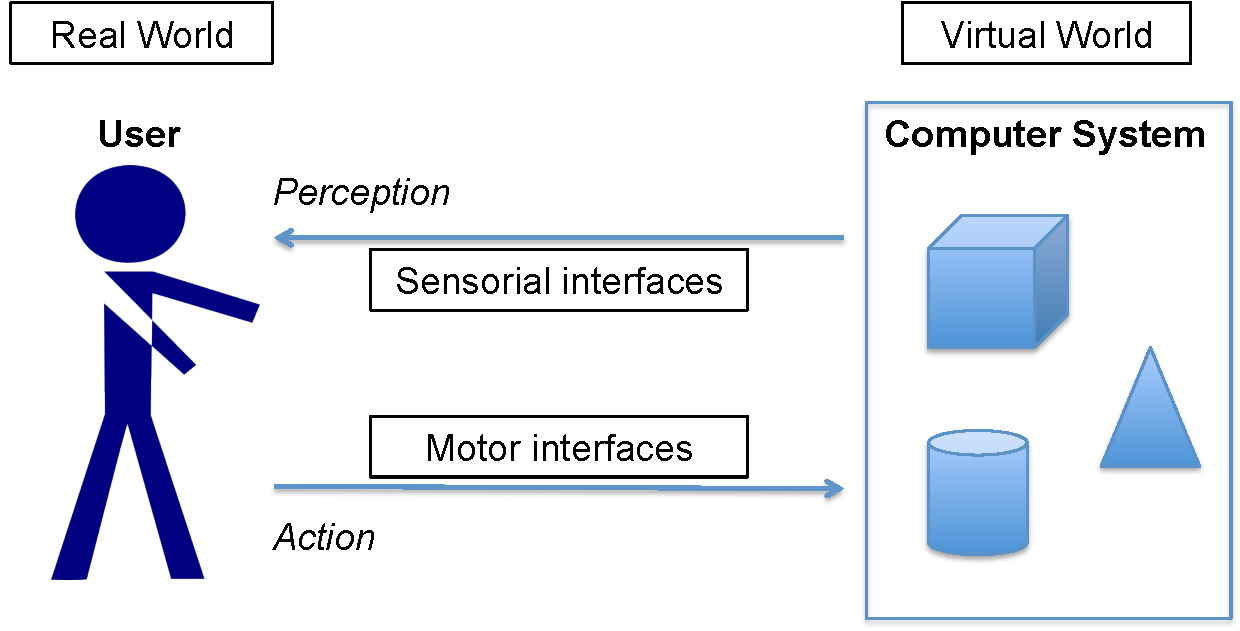
\includegraphics[width=0.9\textwidth]{figures/ch1/loop}
  \caption{\label{fig:1_loop}The ``perception, decision and action" loop in interactive virtual environment.}
\end{figure}

Since the virtual world is totally generated by the computer system, two inherent issues need to be solved: the latency and the sensorimotor discrepancies. The latency is the time lag between the user's action on motor interfaces and the perception of the consequences of this action on the virtual environment through sensorial interfaces. This artifact influences every virtual reality application and may be the source of many problems related to user comfort. The sensorimotor discrepancies is another problem for virtual reality applications. With technical progression, we can simulate more complex phenomenons and provide more interaction through sensorimotor interfaces in the virtual environment, but the real world offers way more information for us to simulate with current technology and the sensorimotor discrepancies will continue to exist.   

Last and the most important point is that, virtual reality possesses two key characteristics which distinguish itself with other existing technologies: immersion and real time interaction.


\subsection{Virtual Environment}
A virtual environment is a computer-generated space.
According to \citet{Fox2009Guide}, a virtual environment (VE) is a digital space in which a user's movements are tracked and his or her surroundings rendered, or digitally composed and displayed to the senses, in accordance with those movements.



\subsection{Immersion and Presence}
Immersion describes the extent to which the virtual stimuli takes the place of real world stimuli within the virtuality continuum.
Immersive virtual environment can maintain several sensory modalities such as visual, audio and haptic to give the users the illusion of ``being there" or the feeling of presence.

Projection-based VR displays, especially systems with Immersive Projected Technologies (IPT) like stereoscopic image walls or CAVEs \citep{CruzNeira1993SPV}, 

Head-Mounted Displays (HMDs) \citep{Melzer1997HMD}, as the name indicates, is a helmet containing two separated displays that are put directly in front of user's eyes allowing visual immersion.

As a key component in virtual reality system, 
Studies have shown that immersion, which can invoke the feeling of presence \citep{Slater1994DepthPre}, has not only a pronounced effect on user performance \citep{Dangelo2008Benefits}, but also has an impact on the social relationship between collaborators \citep{Slater2000Small}.

\citet{Slater1994DepthPre} proposed an important distinction between ``presence" and ``Immersion": presence is a subjective phenomenon such as the sensation of being in a virtual environment, while immersion is an objective description of aspects of the system.
Witmer and Singer relate presence in part to the concept of attention: presence may vary across a range of values that depends in part on the allocation of attentional resources.
They think that both involvement and immersion are necessary for experiencing presence.
Another view of presence is based on the ecological theory of perception \citep{Gibson2014Ecological}.
It suggests that the environment offers situated affordances and there is a perception-action coupling: An organism perceives its environment in terms of its affordances, making perception dependent on possible action.

These definitions don't necessarily contradict with each other, but they can have different implications.
In order to refine these definitions, we need better instruments to measure them.
However, the way that presence is measured depends on the theory that is used, so different approaches are used for the measurement of presence.

The most commonly used measures are based on subjective rating through questionnaires.
\citet{Usoh2000Using} have a questionnaire based on their exclusive presence while \citet{Witmer1998MPV} have another one based on attention involvement. \citet{Schuemie2001Pres} make a taxonomy for different measures of presence and a detailed analysis of factors that influence presence in the virtual environment.

All these theories and measurements can help us to study presence for collaborative immersive interactions, so as to answer questions like: how to be present in the immersive remote world? How to manage the awareness of the others (social presence \citep{Mantovani1999Real})? How to manage the affordances of the scene, including human avatars?
The answers to these questions can help us to make a further step towards the realization of a totally immersive CVE which support a higher level of presence.

\subsection{Interaction}
Providing a good interface for interaction is one of the key aspects for the design of new methods and applications in CVEs.
\citet{Bowman2004UIT} classify interaction with virtual environments as the follows:

\begin{itemize}
\item selection
\item manipulation
\item navigation
\item symbolic input
\item system control
\end{itemize}


\subsection{Summary}

\section{Collaboration}
Collaborative Virtual Environment (CVE) refers to a virtual environment that can be shared by participants connected by a computer (remote or local) network. A collaborative virtual environment (CVE) \citep{Benford2001CVE} enables multiple users to interact \citep{Schroeder2006Usability} and to achieve collaborative tasks \citep{Dodds2009Using} within the same virtual environment. Users can be co-located in the same place or connected remotely.

Users are connected with the virtual world through graphic embodiments called avatars.



\subsection{Typology}

\subsection{User-related Factors}

\subsubsection{User Representation}
Avatars or virtual humans have long been used as virtual representation of the users, or we can call it user embodiment \citep{Benford1995UEC}. Avatars can provide various important functions in a multi-user virtual environment \citep{Thalmann2001VHR}. For example, a user can get other users' positions, focus of interest and see what they are doing, etc. Users can also get a representation of self in the virtual environment by using self-avatars \citep{Lok2003Effects}, which may be especially useful when working with HMDs. Moreover, according to the task that the users need to achieve in the virtual context, social representation of self may be provided through dedicated virtual clothings and/or virtual tools. In an immersive virtual environment, avatars can play a crucial role for user interaction and communication \citep{Slater1994Body}. Users work together not only in a shared virtual world, but also in a shared social space where social human communication is conveyed by avatars \citep{Roberts2004SSH}.

Several techniques can be used to bring avatars to life. In a desktop configuration, we can use input devices like keyboards to activate predefined animations. While in an immersive virtual environment, real time motion capture systems such as Kinect or optical tracking devices are more suitable to map user's physical motion to an avatar \citep{Mohler2010Effect, Vera2011AugMir, Normand2012FBA}. Due to technology limitations or high cost, humanoid avatars do not commonly support facial expression and other subtle social cues. Another interesting method developed by \citet{Ogi2001SteAva} introduces a fully animated video avatar based on live video capture. \citet{Beck2013IGG} used a similar technique to enable interactions between multiple co-located users and a group of remote users by their avatars.

\subsubsection{User Communication}
Social Human Communication

Spatial Communication (Spatial Reference Frame)

\subsubsection{User Interface}
\paragraph{Co-manipulation}
\paragraph{Co-navigation}

\subsubsection{From Presence to Co-presence}



\subsection{Technical Issues}
Collaborative Virtual Environment

Network Architecture, Scene Management, Data Distribution

\subsection{Summary}


\section{Conclusion}

